\documentclass[11pt,a4paper,titlepage,dvipdfmx]{jarticle}
\usepackage{geometry}
\geometry{left=25truemm,right=25truemm,top=25truemm,bottom=37truemm}
\usepackage{ascmac}
\usepackage{multirow}
\usepackage{diagbox}
\usepackage[dvipdfmx]{graphicx}
\usepackage{float}
\usepackage{amsmath,amssymb}
\usepackage{listings,jlisting}
\usepackage{url}
\renewcommand{\lstlistingname}{プログラムリスト}
\renewcommand{\labelenumii}{\arabic{enumii}).}
\lstset{
  basicstyle={\ttfamily},
  identifierstyle={\small},
  commentstyle={\smallitshape},
  keywordstyle={\small\bfseries},
  ndkeywordstyle={\small},
  stringstyle={\small\ttfamily},
  frame={tb},
  breaklines=true,
  columns=[l]{fullflexible},
  numbers=left,
  xrightmargin=0zw,
  xleftmargin=3zw,
  numberstyle={\scriptsize},
  stepnumber=1,
  numbersep=1zw,
  lineskip=-0.5ex
}
\title{\huge{画像処理}}
\author{電子情報工学科5年 \\学籍番号:17404}
\date{提出日:2021年12月20日}

\begin{document}
  \maketitle

  \section{目的}
    本科目達成度の確認のため課題を提出する。
  \section{予備知識}
    本課題では用いる画像はすべてラスター形式の画像である。特に無圧縮のBMP形式を用いる。BMP形式ではヘッダと呼ばれるファイル自体の情報などが
    記載された部分がある。本課題では各ピクセルの画素値の情報のみが必要であるためヘッダを削除する必要がある。ヘッダを削除したファイルのINC形式として
    作成した変換プログラムによって画素値を変換する。その後取り除いたヘッダを追加することで既存の画像ビューアソフトによって閲覧することができる。
    図\ref{fig:flow}に一連の処理の流れを示す。
    \begin{figure}[H]
      \centering
      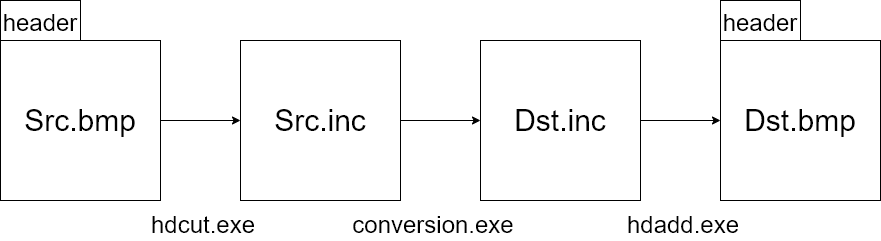
\includegraphics[scale=.4]{./flow.png}
      \caption{画像変換の処理}
      \label{fig:flow}
    \end{figure}
  \section{課題1}
    本章では課題1について課題内容、結果およびプログラムを示す。
    \subsection{課題内容}
      次に課題内容を示す.
      \begin{itembox}[l]{課題1}
        画像処理のデータ変換において,次の変換の入力と出力の関係を表す各関数をグラフで表せ.
        \begin{enumerate}
          \item 輝度調整
          \item 等輝度線
        \end{enumerate}
      \end{itembox}
    \subsection{理論}
      本課題では入力画像としてグレースケール画像を用いる。そのため1ピクセルごとにその濃度値を何らかの関数によって変換する。
      式\eqref{eq:brightnessControl}に輝度調整の変換関数を示す。MAX,MINは指定する閾値である。
      \begin{equation} \label{eq:brightnessControl}
        f(x) = 
        \begin{cases}
        0   &   x < \text{MIN}  \\
        \frac{255(x - \text{MIN})}{\text{MAX} - \text{MIN}} & \text{MIN} \leqq x \leqq \text{MAX} \\
        255        &  x > \text{MAX} 
        \end{cases}
      \end{equation}
      式に等輝度線の変換関数を示す。RANGEは等輝度とみなす輝度幅である。
      \begin{equation} \label{eq:isohighlightLine}
        f(x) = 
        \begin{cases}
        0   &   x < \text{MIN}  \\
        \frac{255(x - \text{MIN})}{\text{MAX} - \text{MIN}} & \text{MIN} \leqq x \leqq \text{MAX} \\
        255        &  x > \text{MAX} 
        \end{cases}
      \end{equation}
    \subsection{結果}

\end{document}